\documentclass[oneside]{book}
\usepackage[utf8]{inputenc} %%\usepackage[utf8x]{inputenc} 
\usepackage[danish]{babel} % Danish letters 

\usepackage{hyperref} % hyperlinks
\usepackage{parskip} % Disable US-type paragraph

\usepackage{afterpage}

\usepackage{listings}
\usepackage{color}

\usepackage[cm]{fullpage}
\usepackage[top=1in, bottom=1.5in, left=1in, right=1in]{geometry}

\usepackage{graphicx}

\definecolor{dkgreen}{rgb}{0,0.6,0}
\definecolor{gray}{rgb}{0.5,0.5,0.5}
\definecolor{mauve}{rgb}{0.58,0,0.82}

\lstset{frame=tb,
  language=sh,%bash,
  aboveskip=3mm,
  belowskip=3mm,
  showstringspaces=false,
  columns=flexible,
  numbers=none,
  numberstyle=\tiny\color{gray},
  breaklines=true,
  breakatwhitespace=true
  tabsize=2
}

\title{Introduktion til Terminal}
\author{Lars Nielsen \\ \href{mailto:lnc13.lars@gmail.com}{lnc13.lars@gmail.com}}
\begin{document}
\maketitle
	\afterpage{\null\newpage}
	\pagenumbering{gobble}
	\clearpage
	\pagenumbering{roman}
	\chapter*{Forord}
Denne bog er tiltænkt nybegynder (n00bz) inden for *NIX\footnote{*NIX er UNIX eller Linux baseret systemer} verden. 
Som godt kunne tænke sig at få en introduktion i hvad der ligger under den poleret brugergrænseflade. 

\section*{Om forfatteren}
Lars er født i 1989 så et lævn fra det forige årtusind. Lars er uddannet datamatiker fra Aarhus Erhvervs Akademi sommeren 2013. 
Men han start med at læse datalogi ved Aarhus Universitet i 2009, men det var nu lidt for teoretisk, så han skiftet til den mere praktisk 
tilgang og læser nu software ved Aalborg Universtet under School of information and computer technology. Desuden har Lars arbejdet ved flere 
virksomheder der udarbejder webbaseret løsninger og nogle få virksomheder der arbjeder primært med back-end løsnigner. Kort sagt Lars er nørd, 
og bruger det mest af sin tid med softwareudvikling og primært ligger hans interesse inden for back-end, system udvikling og systemhåndtering. 

\section*{Kontakt:}
Hvis du har kommentar, forslag eller andre ting til denne bog, ville det være at fortrække at smide en kommentar på bogens github side, 
som findes her \href{https://github.com/looopTools/intro\_til\_terminal}{github.com/looopTools/intro\_til\_terminal}. Hvor der findes en issue side, 
hvor sådanne ting bliver håndteret. Har du derimod et sprøgsmål til Lars selv kan du kontakt ham på følgende mail adresse: \href{mailto:lnc13.lars@gmail.com}{lnc13.lars@gmail.com}

\section*{Tak til:}
Tak til \href{https://www.linux.dk}{www.linux.dk} og holdet bag, for at give mig 
lov til at bruge siden til at start min serie af guides, som er blevet samlet til den her bog. 
\par Tak til Peter Lyberth og Kim Rostgaard Christensen, som begge står bag linux.dk og som af og til har læst nogle af online guidesne igennem, for stavefejl.
\par Tak til folkne bag \LaTeX, som bogen er opbygget i. 
	
	\tableofcontents
	\pagenumbering{gobble}
	\clearpage
	\setcounter{page}{1}
	\pagenumbering{arabic}
	\chapter{Introduktion}
%Det at kunne benyttet sig af kommandolinjen på flere operativ systemer, er en rigtigt god evne. Da de flest systemer tilbyder mindst en form for kommandolinjeværktøj. De systemer som benytte kommandoer som bliver brugt i denne bog høre til familierne; BSD, Mac OS X \& Linux.
%\par Denne bog er henvendt til nybegynder og bygger ens kendskab til kommandoer, på en form som gerne skulle gøre en i stand til at benyttet kommandolinjen på daglig basis.
Terminal eller Terminalen er et kommandolinje værktøj som findes i forskellig udgaver, mmen de flest systemer bruger de samme kommandoer. De kommandoer som bliver brugt i denne bog kan bruges på Mac OS X, Linux og BSD, hvis en funktion ikke findes på alle systemer bliver dette naturligvis noteret.
%\begin{lstlisting}
%cd /Users/test
%\end{lstlisting}
	\chapter{Navigering i filsystemet}
En af de vigtigts ting at kunne i kommandolinjen, er at  havde evnerne til at navigere OS'ets filsystem. Derfor starter vi med at forklare de forskellig kommandoer til at finde rundt.
%\section{Lidt om fil systemet i UNIX}
\section{PWD - hvor er vi?}
En ret relevant dele af navigering er ofte at vide hvor man i det hele taget er. Det er her kommandoen \textit{pwd} kommer ind i billedet. \textit{pwd} står for \textbf{P}rint \textbf{W}orking \textbf{D}irectory, kommandoen returnere den sti som man arbejder i lige nu. 
\begin{lstlisting}
	h271:intro_til_terminal tools $ pwd
	/Users/tools/Documents/intro_til_terminal
\end{lstlisting}
\subsection*{Og hvad så}
Hvad kan man så bruge det til? Man kan altid bruge ens nuværende "position" til at navigere filsystemet. Men for at kunne bruge information skal man kunne forstå resultat, så lad os bryde stien ned. 
\subsubsection*{intro\_til\_terminal}
Det sidste element af stien er den mappe, man arbejder i og interager med. Det er altså her andre kommandoer som interagere med filer og visse andre kommandoer udføre deres arbejde hvis de bliver kaldt. %forklar kaldt
\subsubsection*{/Users/tools/Documents/}
Er den overordnet filsti, som man er nød til at komme igennem for at kunne komme til \textit{intro\_til\_terminal}.

\section{LS - Hvad er der her?}
En anden vigtigt del af at arbejde i filsystemet, er at vide hvilke filer og mapper, som er i den mappe man arbejder i. Det er til dette formål man bruger kommandoen \textit{ls}. \textit{ls} betyder list directory contents, altså list indholdet af en mappe. Hvis kommandoen kaldes ud flag, returneres en liste af alt, som ikke er skjult i mappen.
\begin{lstlisting}
	h271:intro_til_terminal tools$ ls
	LICENSE		fil_sys_nav.tex	intro.tex	main_book.tex
	README.md	forord.aux	main_book.aux	main_book.toc
	compile.sh	forord.tex	main_book.log	ordliste.aux
	fil_sys_nav.aux	intro.aux	main_book.pdf	ordliste.tex
\end{lstlisting}
\subsection*{Men jeg har skjulte filer}
På UNIX baseret, systemer er alle filer og mapper som starter med \textit{.} skjulte, eksemplet kunne hede .skjult. Den vil vi altså gerne kunne se, så vi bruger flaget \textit{-a} som står for all eller alle, også får man en lidt anderledes liste returneret.
\begin{lstlisting}
	h271:intro_til_terminal tools$ ls -a
	.		LICENSE		fil_sys_nav.tex	intro.tex	
	..		README.md	forord.aux	main_book.aux	
	.git		compile.sh	forord.tex	main_book.log	
	.skjult		fil_sys_nav.aux	intro.aux	main_book.pdf	
\end{lstlisting}
\subsection*{List alt i en undermappe}
Man kan også liste alt i mappe ved at give stien til mappe
\begin{lstlisting}
  h271:test tools$ ls
  t_1    t_2    test_2
  h271:test tools$ ls t_1
  demo.txt
\end{lstlisting}
\section{CD - Jeg vil væk}
For at kunne navigere rundt i sit filsystem skal man naturligvis også kunne komme væk fra den mappe man er i. Dette gøres via kommandoen \textit{cd}, som står \textbf{C}hange \textbf{D}irectory eller ændre mappe. 
\begin{lstlisting}
	h271:intro_til_terminal tools$ pwd
	/Users/tools/Documents/intro_til_terminal
	h271:intro_til_terminal tools$ cd test/
	h271:test tools$ pwd
	/Users/tools/Documents/intro_til_terminal/test
\end{lstlisting}
Hvis man vil et "trin" op i filsystemet skriver man \textit{cd ..}
\section{MKDIR - Ny mappe}
Man kan få brug for oprette en mappe, dette gøres med kommandoen; \textit{mkdir} som betyder \textbf{M}a\textbf{K}e \textbf{Dir}ectory eller lav mappe. Kommandoen opretter en mappe i den nuværende arbejdesmappe.
\begin{lstlisting}
	h271:test tools$ pwd
	/Users/tools/Documents/intro_til_terminal/test
	h271:test tools$ ls
	h271:test tools$ mkdir test_2
	h271:test tools$ ls
	test_2
\end{lstlisting}
\section{CP - Kopi}
Hvis man ønsker at kopiere en fil, gøres dette med kommandoen \textit{cp} som står for \textbf{C}o\textbf{p}y. Kommandoen kræver 2 argumenter; filen som ønskes kopieret og destinations mappen. Så hvis man har en mappe \textit{t\_1} som indholder en fil \textit{demo.txt} som man ønsker at flyttet til mappen \textit{t\_2} gøres det sådan her:
\begin{lstlisting}
	h271:test tools$ ls t_1
        demo.txt
	h271:test tools$ ls t_2
	h271:test tools$ cp t_1/demo.txt t_2
	h271:test tools$ ls t_1
        demo.txt
	h271:test tools$ ls t_2
        demo.txt
\end{lstlisting}
\section{MV - Flyt dig}
\textbf{M}o\textbf{V}e eller flyt er en måde hvor på man kan flytte en fil eller en mappe fra et sted i systemet til et andet. Lige som \textit{cp} tager \textit{mv} to argumenter, elementer som man vil havde flyttet og destinations mappen. 
\begin{lstlisting}
	h271:test tools$ ls t_1
        demo.txt
	h271:test tools$ ls t_2
	h271:test tools$ mv t_1/demo.txt t_2/
	h271:test tools$ ls t_1
	h271:test tools$ ls t_2
        demo.txt
\end{lstlisting}
\subsection*{Omdøb}
Man kan også omdøbe en fil med kommandoen \textit{mv}, dette gøres ved at tage en fil som først parameter og bruger en fil som anden parameter, eksempeltvis
\begin{lstlisting}
	h271:t_2 tools$ ls
        demo.txt
	h271:t_2 tools$ mv demo.txt demo_2.txt 
        :t_2 tools$ ls
        demo_2.txt
\end{lstlisting}
\section{RM - Væk med dig}
\textbf{R}e\textbf{M}ove eller fjern er en kommando som kan bruges til at slette filer. 
\begin{lstlisting}
	h271:test tools$ ls t_2/
        demo_2.txt
	h271:test tools$ rm t_2/demo_2.txt 
	h271:test tools$ ls t_2/
\end{lstlisting}
\subsection*{-r fjer alt under mig og mig}
Hvis man ønsker at slette en mappe og alt der ligger i mappen, skal man sætte følgende flag på \textit{rm -r}, hvor \textit{-r} står for rekrusiv. Hvilket vil sige at den udføre kommandoen rekrusivt.
\begin{lstlisting}
	h271:test tools$ ls
        t_1	t_2	test_2
	h271:test tools$ ls test_2/
        demo_2.txt
	h271:test tools$ rm -r test_2/
	h271:test tools$ ls
        t_1	t_2
\end{lstlisting}
\subsection*{RMDIR - Fjern mappe med indhold}
Hvis man vil fjerne en mappe, som man ved er tom, kan man skrive \textit{rmdir} og så mappens navn som argument.
\begin{lstlisting}
	h271:test tools$ ls
        t_1	t_2
	h271:test tools$ ls t_2
	h271:test tools$ rmdir t_2/
	h271:test tools$ ls
        t_1
\end{lstlisting}

	\chapter{Så kikker vi på diske}
I dette kapitel kikkes der på, hvordan man får overblik over, hvor meget plads der er på ens interndisk og eksterndiske, pluds lidt små sjov ting
omkring diske.
\section{df - fri disk}
\textit{d}isk \textit{f}ree informere dig om hvor meget plads der bliver brugt på din disk og hvor meget der er frit på disken.
For at benytte kommandoen indtastes simpelthen bare \textit{df}
\\
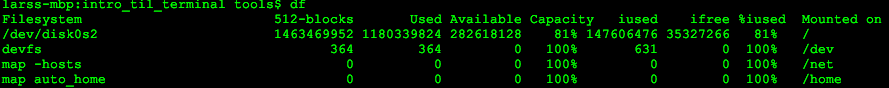
\includegraphics[scale=0.55]{images/df_std.png}
\subsection{-h - Menneskligt læsligt}
Som kan ses på outputtet i billedet her over, er outputet ikke videre forståeligt, for ikke teknisk folk. Men \textit{df} har et flag som er \textit{-h}, som giver et bedere og mere læsbar output og kaldes således \textit{df -h}.\\
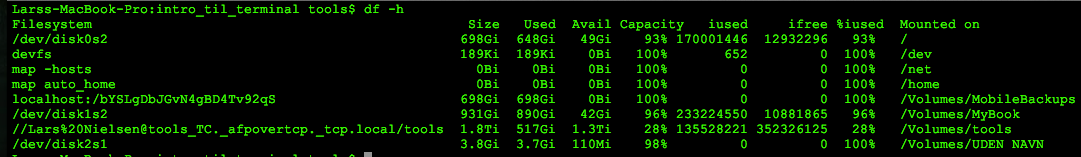
\includegraphics[scale=0.45]{images/df_h.png} 

        \chapter{Historie}
Hvis man ofte bruger samme kommando med samme pararmeter, eller ikke lige kan huske hvordan en kommandos struktur den er, kan du bruge kommandoen \textit{history}
\begin{lstlisting}
	h271:intro_til_terminal tools$ history
	  495  sudo rm /etc/postgres-reg.ini
	  496  brew list
	  497  brew update
	  498  brew install postgresql
	  499  sudo port install postgresql93
	  500  sudo port selfupdate
	  501  cd Documents/intro_til_terminal/
	  502  ls
	  503  open main_book.pdf 
	  504  clear
	  505  history
	h271:intro_til_terminal tools$ 
\end{lstlisting}
Dette er som det kan ses et meget lille udsnit af alle kommandoer, man kan scrolle igeenem sin historier. Her kan man så se tideliger kommandoer man har kaldt. 
\subsection*{Kald mig igen}
Som det kan ses i outputet ovenen for har være kommando fået tildelt et nummer, eksempeltvis har \textit{ls} fået nummer 502. det nummer er ret behjælpligt hvis man ikke ønsker at indtastet hele kommandoen igen, så kan man i stedet for indtaste \textit{!nummer} og så bliver kommandoen kørt igen, Men man skal være opmærksom på at tallet ændre sig, som kommandoerne bliver skubet ud af historien. 
\begin{lstlisting}
	h271:intro_til_terminal tools$ !502
	 ls
	 #compile.sh#	disk.tex	hist.aux	main_book.aux	mkdir
	 #hist.tex#	disk.tex~	hist.tex	main_book.log	ordliste.aux
	 LICENSE		fil_sys_nav.aux	hist.tex~	main_book.out	ordliste.tex
	 README.md	fil_sys_nav.tex	images		main_book.pdf	test
	 compile.sh	forord.aux	intro.aux	main_book.tex
	 disk.aux	forord.tex	intro.tex	main_book.toc
	h271:intro_til_terminal tools$ 
\end{lstlisting}


        \chapter{Processer}
Som de flest ved hvis de kommer fra eksempeltvis Windows eller Mac OS X, kan man se hvilke processer der køre via en jobliste på *nix systemer kan dette også gøres via kommandolinje og man kan også dræbe de processer som er løbet løbsk.
\section{TOP hvad kører}
Top hviser de mest belastne processer der køre og lidt informaiton om forskellig ting. Kommandoen kaldes ved at skrive \textit{top} og følgende output bliver vist  
\begin{lstlisting}
	h271:intro_til_terminal tools$ top
Processes: 188 total, 3 running, 4 stuck, 181 sleeping, 832 threads    11:22:47
Load Avg: 1.55, 1.62, 1.67  CPU usage: 10.8% user, 14.47% sys, 75.43% idle
SharedLibs: 175M resident, 0B data, 35M linkedit.
MemRegions: 39816 total, 2761M resident, 130M private, 770M shared.
PhysMem: 5441M used (1216M wired), 2750M unused.
VM: 454G vsize, 1310M framework vsize, 0(0) swapins, 0(0) swapouts.
Networks: packets: 2348958/2325M in, 2145578/1783M out.
Disks: 2436784/21G read, 207259/6427M written.

PID   COMMAND      %CPU      TIME     #TH  #WQ  #PORT #MREG MEM    RPRVT  PURG
4362  mdworker     0.0       00:00.09 4    0    54    58    1976K  1084K  0B
4152  top          11.7      00:34.09 1/1  0    23    35    2244K  2020K  0B
4149  com.apple.au 0.0       00:00.03 2    1    48    53    1328K  648K   0B
4148  com.apple.au 0.0       00:00.01 2    1    28    42    1004K  444K   0B
4147- com.apple.qt 0.0       00:00.07 2    0    73    81    2956K  1452K  0B
4146  com.apple.We 0.0       00:03.40 9    0    243   557   44M    40M    72K
4129  com.apple.Co 0.0       00:00.01 2    1    30    41    956K   400K   0B
4122  com.apple.Pr 0.0       00:00.01 2    1    35    42    980K   412K   0B
4119  Preview      0.0       00:06.53 4    0    205   444   35M    38M    20M
3926  Twitter      0.0       00:03.23 8    1    223   744   59M    47M    196K
3920  com.apple.hi 0.0       00:00.01 2    0    31    38    916K   368K   0B
3919- com.apple.qt 0.0       00:00.08 2    0    72    81    2932K  1428K  0B
3918  com.apple.We 3.9       00:23.06 11   2    267   1249+ 127M+  110M+  692K
3836  ScopedBookma 0.0       00:00.07 2    1    40    43    1800K  1360K  0B
\end{lstlisting}
\section{KILL og PKILL}
\textit{kill} og \textit{pkill} bruges til at dræbe processer, men på to forskellig måder.
\subsection*{KILL}
Basere sig på en nummer som kaldes \textit{PID} som er en process id, og som kan ses i outputtet for top. Alle processer har et \textit{PID} og de er alle unik (det vil sige ikke to er ens). Det at der er unikke tillader at man kan bruge \textit{kill} til at dræbe en process, lad os dræb Twitter processen som har PDI: 3926 
\begin{lstlisting}
	h271:intro_til_terminal tools$ kill 3926
\end{lstlisting}

\subsection*{PKILL - Vi dræber på navn}
Man kan også dræbe en process via dens kommando navn, så hvis man lige som under \textit{kill} vil dræbe Twitter kan det gøres således med \textit{pkill}
\begin{lstlisting}
	h271:intro_til_terminal tools$ pkill twitter
\end{lstlisting}
Med \textit{pkill} skal man være lidt mere påpasselig, da der godt kan køre flere processer med samme kommando navn. Der for anbefales det at man som nybegynder benytter \textit{kill}.


        \chapter{Små gode ting}
I dette kapitel dækkes små "hacks" til at kunne gøre arbejdet med kommandolinjen letter.
\section{Mange kommandoer på engang}
Når man med tiden opdager at flere kommando tit bliver ud ført sammen og i hvis række følge, bliver man træt af at skrive en kommando trykke enter og så skrive næste kommando, og det er her man bliver glad for \textit{\&\&} som tillader en at link kommandoer.
Eksempelvis, hvis man vil lave en mappe også gå direkte ind i den, altså kombinere \textit{mkdir} og \textit{cd}, og i dette eksempels tilfælde også \textit{pwd} kan dette gøres så ledes .
\begin{lstlisting}
	h271:intro_til_terminal tools$ pwd && mkdir kombi_test && cd kombi_test && pwd
	  /Users/tools/Documents/intro_til_terminal
	  /Users/tools/Documents/intro_til_terminal/kombi_test 
\end{lstlisting}
Som udføre alle kommandoerne i række følge. 
\section{ALIAS}
Kommandoer kan være lange og svære og huske, derfor kan man benytte benytte sig af \textit{alias}.
Alias er i sig selv ikke kommando men en funktionalitet, som er en del af ens kommandolinjeværktøj. 
For at benyttet sig af alias, skal der editeres i en fil som kaldes \textit{.bashrc}, denne fil 
kan editeres ved at benytte \textit{VI}. Som eksempel, vil vi benytte kommandoen cd som eksempel, 
også vil vi gerne ændre nuværende mappe til skrivebordet, vi gør så ledes:
\begin{lstlisting}
	h271:intro_til_terminal tools$ vi  ~/.bashrc
\end{lstlisting}
Når \textit{VI} åbnes skal man trykke \textit{i} for at indsætte de tegn der er behov for og på en ny linje nederst, i file skrives:
\begin{center}
  alias cddesktop='cd ~/Desktop'
\end{center}
For at gennem trykkes der på escape knappe (esc), og så følge \textit{:wq}. \textit{:wq} er en vi kommando, w = write, q = quit. Når man har gemt, skal man genilæse sing \textit{.bashrc} fil, dette gøres således:
\begin{lstlisting}
	h271:intro_til_terminal tools$ .  ~/.bashrc
\end{lstlisting}

\section{CURL}
I dette afsnit benyttes material fra \href{http:www.ruby-lang.org}{www.ruby-lang.org} \par
CURL er en måde hvor på en fil kan hentes fra en server, det gøre ret simpelt med \textit{curl \#adresse til filen på serveren\#}, men outputtet giver ikke altid mening. Derfor kan man gøre brug af flaget -O, som gør at filen kan gives et navn. kommandostrukturen ser således \textit{curl \#navn\_på\_fil\# \#adresse til filen på serveren\#} og man skal være i den mappe, man ønsker filen skal ligge, eller give stien ved fil navnet. Se eksempel neden for 

\begin{lstlisting}
	h271h271:curl tools$ ls
	h271:curl tools$ curl -o ruby-2.1.0.tar.gz http://cache.ruby-lang.org/pub/ruby/2.1/ruby-2.1.0.tar.gz
	    % Total    % Received % Xferd  Average Speed   Time    Time     Time  Current
	                                   Dload  Upload   Total   Spent    Left  Speed
          100 14.3M  100 14.3M    0     0  6368k      0  0:00:02  0:00:02 --:--:-- 8655k
	h271:curl tools$ ls
	  ruby-2.1.0.tar.gz
\end{lstlisting}
\section{grep}
Grep tillader søgning i tekst filer, og kommandoen kaldes ved at skrive 
\textit{grep søgeord filnavn} og man får som retur de linjer i teksten hvor der står det ord man søger efter
\begin{lstlisting}
	h271:intro_til_terminal tools$ grep grep mange.tex
	Greb tillader soegning i tekst filer, og kommandoen kaldes ved at skrive \textit{grep #file\_name#}
\end{lstlisting}

	\appendix
	\chapter{Ordliste}
Da ikke alle benytter de samme ord for alt, er der her en ordlist, som forklare ordne som bliver brugt.
\begin{description}
   \item[Mappe] et element som kan indeholde andre mapper og filer. Kaldes også for folder. 
   \item[*NIX] er et gennerelt udtryk for systemer som basere sig på UNIX og GNU/Linux 
   \item[*BSD] er en familie af UNIX baseret systemer som bygger på BSD eller Berkely 
     Software Distrobution, familiemedelmmer er blandt andre Mac OS X, FreeBSD og OpenBSD.
   \item[OS X og Mac OS X] er det system som Apple Inc. benytter på deres bærebare 
     og stationære computer. OS X er delvist baseret på NextSTEP og FreeBSD.
   \item[Parameter] disse kaldes også argumenter, men i denne bog brugers argumenter om noget andet.     
   \item[Dash (-)] kaldes normalt bindestreg. 
\end{description}

\end{document}
